\section{Proposta}

Este trabalho tem como proposta a utilização de um modelo de inteligência artificial para segmentação panóptica que irá classificar os pixeis na imagem e permitir que os usuários gerem mapas a partir da seleção de um dos segmentos da imagem.

Utilizando o modelo EfficientPS é possível fazer a segmentação panóptica, segue um exemplo na \cref{fig:segmantations_1} e na \cref{fig:segmantations_2}. O modelo citado está disponível no GitHub dos próprios autores \space\citeonline{mohan2020efficientps} e será treinado com a combinação de pelo menos dois conjuntos de dados citados anteriormente. No resultado apenas será identificado os pixeis de classes contidas nos conjuntos de dados escolhidos, portanto é possível que em uma imagem não seja identificado nada:

\begin{figure}[!ht]
	\centering
    \caption{Imagem de entrada para rede neural.}
	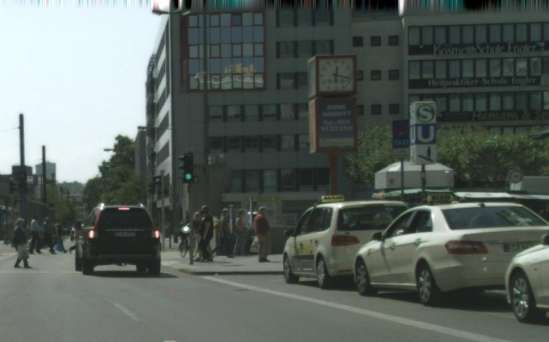
\includegraphics[width=0.6\textwidth]{figures/segmantations_1.png}
    \legend{Fonte: \space\citeonline{kirillov2019panoptic}}
	\label{fig:segmantations_1}
\end{figure}

\begin{figure}[!ht]
	\centering
    \caption{Imagem saída de um modelo de segmentação panóptica de segmentação panóptica.}
	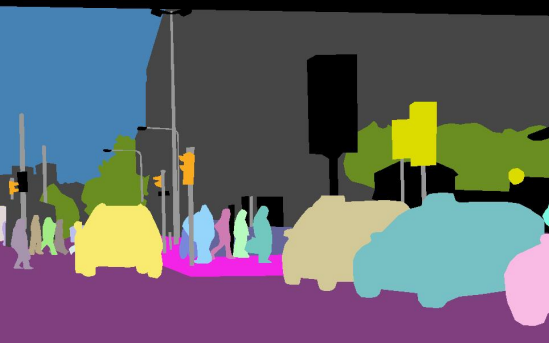
\includegraphics[width=0.6\textwidth]{figures/segmantations_2.png}
    \legend{Fonte: \space\citeonline{kirillov2019panoptic}}
	\label{fig:segmantations_2}
\end{figure}

Após a segmentação da imagem o usuário poderá selecionar qual parte da imagem será utilizada para gerar a ilha.

Feito a seleção será gerado um diagrama de Voronoi que funcionará como um filtro em cima dessa imagem, assim gerando a ilha e os biomas.

\begin{figure}[!ht]
	\centering
    \caption{Ilha gerada a partir da segmentação panóptica e aplicando um filtro com o diagrama de Voronoi, azul representa oceano, verde floresta, cinza montanhas.}
	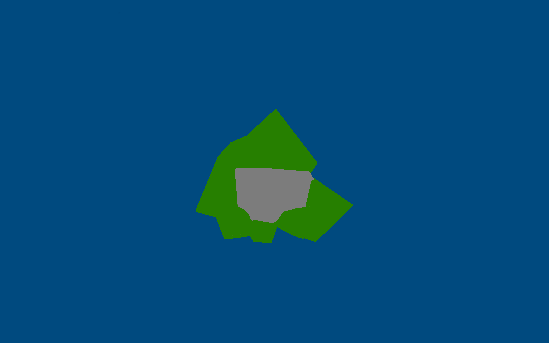
\includegraphics[width=0.6\textwidth]{figures/segmantations_pnl.png}
    \legend{Fonte: Criação própria}
	\label{fig:segmantations_pnl}
\end{figure}

